\documentclass{article}

\usepackage[preprint,nonatbib]{neurips_2025}

\usepackage[utf8]{inputenc}
\usepackage[T1]{fontenc}
\usepackage{hyperref}
\usepackage{url}
\usepackage{booktabs}
\usepackage{graphicx}
\usepackage{amsfonts,amsmath,amssymb}
\usepackage{nicefrac}
\usepackage{microtype}
\usepackage{xcolor}
\usepackage{enumitem}
\usepackage{float}

\newcommand{\smiles}{\textsc{smiles}}
\newcommand{\spectralm}{\textsc{SpectraLM}}

\newcommand\blfootnote[1]{%
  \begingroup
  \renewcommand\thefootnote{}\footnote{#1}%
  \addtocounter{footnote}{-1}%
  \endgroup
}

\title{\spectralm: A Constraint-Aware Text LLM Study of Molecular Structure Prediction from One-Dimensional NMR Peak Tables}

\author{%
  Yubin Xiong\,$^{1\,2}$ \\
  \texttt{kimariyb@163.com} \\
  \And
  Xinchang Wang\footnotemark[1]\;\,${}^{1\,2}$\\
  \texttt{xcwang@xmu.edu.cn} 
}

\begin{document}

\maketitle

\begin{abstract}
One-dimensional \(^{1}\)H and \(^{13}\)C nuclear magnetic resonance (NMR) spectra are among the most routinely available measurements for small-molecule structure elucidation, yet mapping such spectra to a unique molecular graph remains difficult. Recent work has explored transformers, reinforcement learning, diffusion models, and physics-guided search for NMR-based structure elucidation, but it remains unclear what can be achieved by a general-purpose text large language model (LLM) when the spectral input is represented as structured peak tables rather than images or raw arrays. This paper presents \spectralm, a text-only instruction-tuning framework for predicting molecular connectivity from paired \(^{1}\)H/\(^{13}\)C NMR peak tables with an optional molecular formula. The system builds a controlled 10k benchmark, filters molecules to a single neutral isotope-free component over common organic elements, fine-tunes Qwen3-8B adapters with response-only supervision, and evaluates direct JSON-constrained \smiles{} generation and top-\(k\) candidate generation with formula/domain filtering and NMR-rule reranking. The main empirical finding is deliberately modest. The model learns to emit valid molecular strings and partial NMR-to-functional-group associations, but direct exact structure recovery is not yet reliable: on the 1,000-sample test set, formula-conditioned direct generation reaches 94.3\% valid \smiles{}, 65.7\% functional-group micro-F1, 18.3\% mean Morgan Tanimoto similarity, and only 0.2\% exact connectivity match. Formula conditioning improves several soft metrics, but prompt-only formula conditioning is insufficient because molecular formula accuracy remains 2.6\% for direct generation. Candidate generation is limited by recall rather than ranking: top-32 formula-conditioned candidate oracle connectivity is only 0.5\%. These results suggest that text LLMs can learn chemically meaningful local correspondences from 1D NMR peak tables, but exact structure elucidation requires stronger formula-valid candidate generation, retrieval, or chemically constrained decoding before reranking can become effective.
\end{abstract}

\blfootnote{\hspace{-6mm}${}^*$ Corresponding author.}
\blfootnote{\hspace{-6mm}$^{1}$School of Electronic Science and Engineering, Xiamen University, China.}
\blfootnote{\hspace{-6mm}$^{2}$State Key Laboratory for Physical Chemistry of Solid Surfaces, Xiamen University, China.}

\section{Introduction}

Small-molecule structure elucidation is a central problem in organic chemistry, natural product discovery, reaction monitoring, and analytical quality control. Routine one-dimensional NMR spectroscopy is often the first source of structural evidence because \(^{1}\)H and \(^{13}\)C spectra report complementary information about hydrogen and carbon environments \cite{Ernst1987,Levitt2008,Silverstein2014,Claridge2016}. A trained chemist combines chemical shifts, multiplicities, coupling constants, integrations, signal counts, molecular formulae, double-bond equivalents, and prior chemical constraints to propose a structure. This reasoning is powerful, but it is also slow, expertise-dependent, and difficult to scale across large spectral collections.

Automated structure elucidation has therefore become a natural target for machine learning. Earlier data-driven systems framed the problem as substructure prediction followed by candidate ranking \cite{Huang2021,Hu2024}. Other work has used molecular generation or search procedures, including reinforcement learning \cite{Sridharan2022,Devata2024}, conditional molecular generation \cite{Yao2023}, spectral language modeling \cite{Alberts2023,Alberts2025}, diffusion models \cite{Xiong2025,Yang2025}, set transformers \cite{Yang2026}, and large-scale spectral matching with physics-guided optimization \cite{Jin2026}. These studies have substantially advanced automated NMR interpretation, but they also reveal that results depend strongly on the representation, available modalities, molecule size, formula availability, and whether inference is direct generation, database matching, or candidate reranking.

This study asks a narrower and practically useful question: what does a general-purpose text LLM learn when the only model-visible spectral evidence is a structured \(^{1}\)H/\(^{13}\)C NMR peak table, optionally accompanied by a molecular formula? The question matters because peak tables are compact, easy to serialize, and close to how spectroscopists summarize routine 1D NMR evidence. A text-only model is also simpler and faster to train than a vision-language model over rendered spectra. At the same time, a text LLM is not chemically constrained by default. It may generate syntactically valid \smiles{} strings that violate the molecular formula, contain unsupported elements, or correspond to plausible but incorrect isomers. A useful evaluation must therefore measure not only exact matches, but also validity, formula consistency, scaffold similarity, functional-group overlap, output format compliance, and candidate oracle recall.

We present \spectralm, an end-to-end research framework for this text-only setting. The system converts paired NMR samples into deterministic peak-table prompts, trains Qwen3-8B LoRA adapters with JSON \smiles{} targets, and evaluates both direct and candidate-based inference. The framework intentionally separates formula-conditioned and no-formula settings, because molecular formula is an unusually strong constraint in NMR interpretation and should not be confounded with prompt augmentation. It also includes a machine-readable 1D NMR rule library for deterministic evidence generation and post-generation candidate validation. In the experiments reported here, however, the rule library is not injected into the training prompts; this keeps the pilot focused on what the text LLM learns from peak tables and formula alone.

The contribution is not a claim of state-of-the-art accuracy. Instead, this paper reports a controlled negative and diagnostic result. Fine-tuning a text LLM on 10k curated NMR examples produces high valid-\smiles{} rates and meaningful functional-group signal, but exact connectivity recovery remains near zero. Formula conditioning improves soft metrics, yet the model often ignores the formula when it is supplied only as text. Candidate ranking also fails to help because the sampled candidate set rarely contains the reference structure. These observations sharpen the research direction: the next bottleneck is not a better reranker, but a candidate generator or decoding procedure that can produce diverse, formula-valid molecules with substantially higher oracle recall.

Figure~\ref{fig:workflow} summarizes the final research framing. The important design choice is that the LLM is not treated as a stand-alone chemistry engine. It is a conditional text generator embedded inside a chemical validation pipeline. This framing avoids overclaiming what a small instruction-tuned model can infer from ambiguous 1D NMR evidence, while still preserving a useful role for LLMs: flexible prompt conditioning, structured output, auxiliary task learning, and candidate scoring once chemically plausible candidates exist.

\begin{figure}[t]
\centering
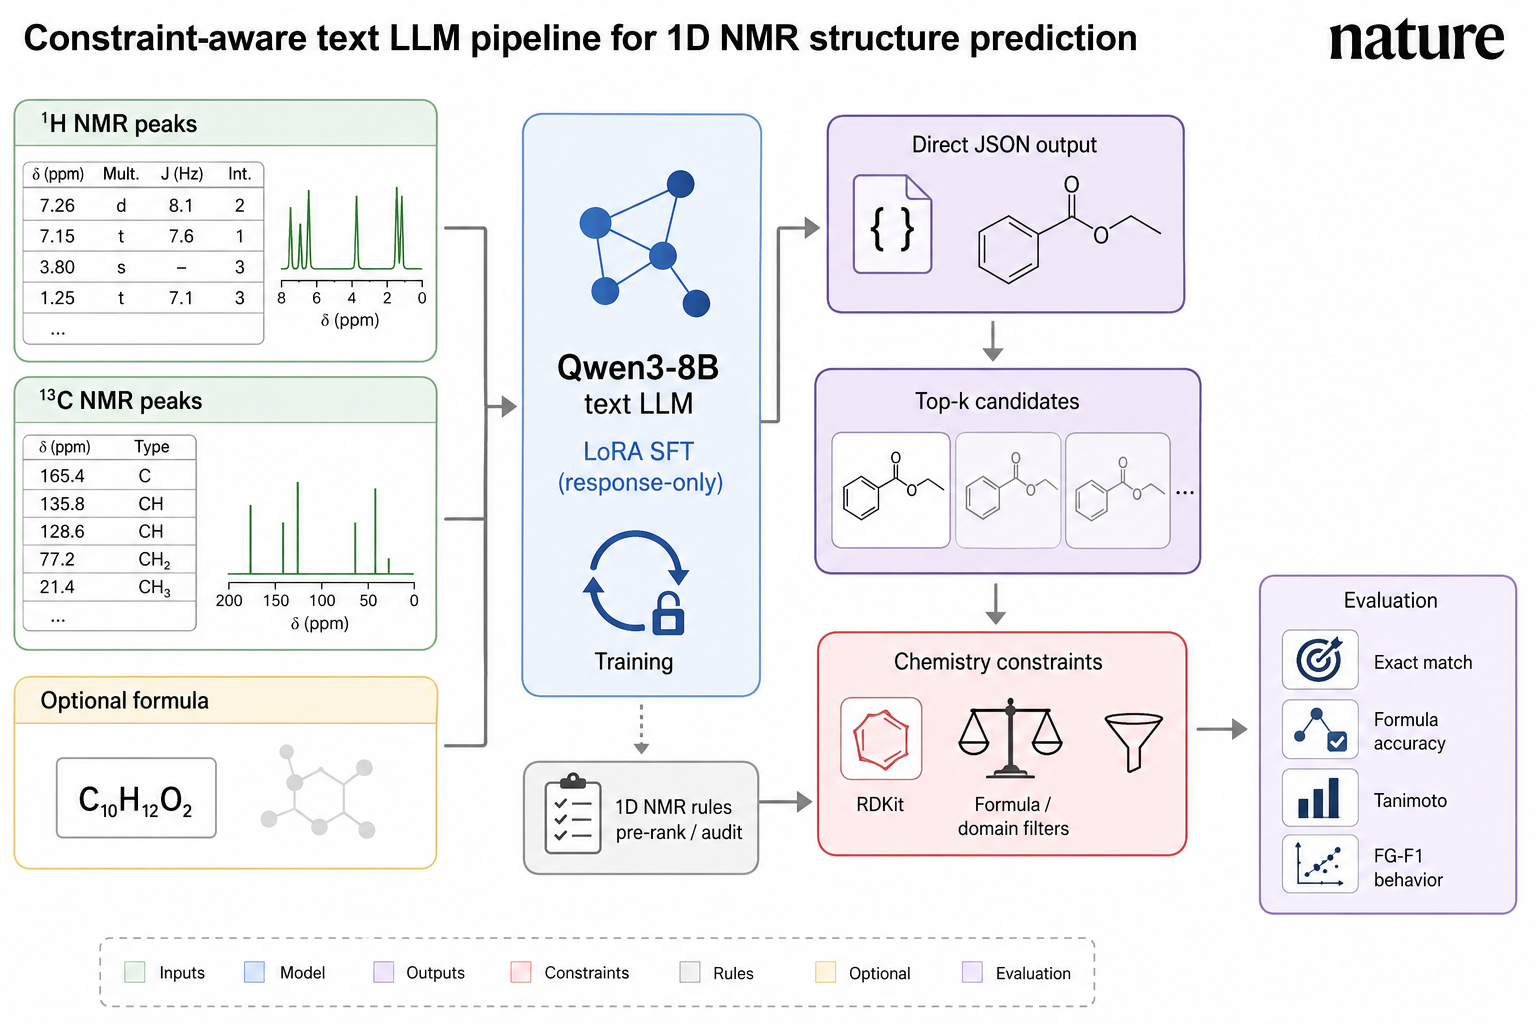
\includegraphics[width=\linewidth]{figures/fig1_workflow.png}
\caption{\textbf{Overview of the text-only \spectralm{} pipeline.} The model receives deterministic \(^{1}\)H/\(^{13}\)C peak tables and an optional molecular formula, then emits either a direct JSON \smiles{} prediction or sampled candidate structures. RDKit validation, formula/domain filtering, and one-dimensional NMR rules are applied outside the model. The central empirical question is where this hybrid pipeline fails: text learning, formula compliance, candidate recall, or reranking.}
\label{fig:workflow}
\end{figure}

\section{Related Work}

\subsection{Machine learning for NMR-based structure elucidation}

Classical NMR interpretation has long relied on human-readable tables of chemical-shift ranges, multiplicity heuristics, integration checks, and unsaturation constraints \cite{Breitmaier2002,Pretsch2009,Claridge2016}. These rules are approximate because chemical shifts depend on solvent, concentration, substituent effects, stereochemistry, and conformational averaging. They are nevertheless useful because they translate raw spectra into local structural evidence: aromatic protons, carbonyl carbons, heteroatom-adjacent methylenes, alkenes, alkynes, nitriles, and other recognizable regions. The present work uses this observation to justify a text representation. A peak table is not merely a lossy substitute for an image; it is close to the intermediate representation used in routine manual analysis.

Several lines of work have explored NMR-to-structure prediction. Huang et al. \cite{Huang2021} proposed an automated structure elucidation framework that predicts substructures from routine 1D NMR spectra and uses them to rank candidate constitutional isomers. Their system achieved strong top-ten candidate recovery for small molecules when molecular formula information was available. Hu et al. \cite{Hu2024} later introduced a multitask framework for one-dimensional NMR that combines spectral processing and molecular assembly, reporting large reductions in chemical search space and strong top-\(k\) performance for molecules up to 19 heavy atoms. These studies support the idea that 1D NMR contains useful structure information, but they also rely on domain-specific modeling and candidate assembly rather than unconstrained sequence generation.

Transformer-based approaches have examined NMR as a language-like signal. Alberts et al. \cite{Alberts2023} trained transformers on synthetic NMR spectra and reported that a model using both \(^{1}\)H and \(^{13}\)C spectra could predict molecular structures with substantial top-1 accuracy under their simulation setting. A later multimodal multitask model integrated NMR and infrared evidence and reported high prediction accuracy after simulated pretraining and experimental fine-tuning \cite{Alberts2025}. These results indicate that spectral modalities can be learned by sequence models, but the setting differs from the present study: \spectralm{} uses a general text LLM, structured peak tables, and a deliberately small pilot cohort to examine feasibility and failure modes.

Other methods treat structure elucidation as search or generation in molecular graph space. Sridharan et al. \cite{Sridharan2022} framed NMR inverse design as a graph-building reinforcement learning problem. Devata et al. \cite{Devata2024} extended this direction with DeepSPInN, using infrared and \(^{13}\)C NMR spectra within a Monte Carlo tree search formulation. Conditional molecular generation from \(^{13}\)C NMR and prior knowledge has also been explored \cite{Yao2023}. More recent approaches use diffusion-style molecular generation from NMR evidence \cite{Xiong2025,Yang2025} or set transformers for experimental NMR peak sets \cite{Yang2026}. NMR-Solver combines large-scale spectral matching with physics-guided fragment optimization \cite{Jin2026}. Compared with these methods, \spectralm{} does not introduce a new molecular graph generator. It asks whether an instruction-tuned text LLM can serve as a direct or candidate generator when paired with hard chemical post-processing.

\subsection{Large language models and constrained molecular generation}

Text LLMs are attractive for chemistry because molecular strings, peak tables, reaction descriptions, and instructions can all be represented as text. Transformers \cite{Vaswani2017} provide the underlying architecture, and open-source training stacks such as PyTorch, Transformers, PEFT, and TRL make instruction tuning reproducible at modest adapter cost \cite{Paszke2019,Wolf2020,Mangrulkar2022,VonWerra2020}. Parameter-efficient methods such as LoRA \cite{Hu2021LoRA} and QLoRA \cite{Dettmers2023QLoRA} make it practical to fine-tune large checkpoints on domain data; the present experiments use a Qwen3 text checkpoint as the base model \cite{QwenTeam2025}. The weakness is that ordinary autoregressive decoding does not enforce graph validity, molecular formula, element policy, charge neutrality, or uniqueness. A valid \smiles{} string \cite{Weininger1988} may still be chemically inconsistent with the input. For NMR, this matters because many incorrect isomers can share broad spectral features, and the molecular formula is often one of the few hard constraints available.

\spectralm{} therefore treats the LLM as only one component of an inference pipeline. The model is trained to emit a strict JSON object with a \texttt{smiles} field. RDKit \cite{RDKit} is then used for canonicalization, formula computation, domain checks, fingerprints, and scaffold analysis. Candidate inference samples multiple outputs, deduplicates them, removes invalid or out-of-domain molecules, and applies formula filtering when a formula is provided. This design reflects a general principle: when the output object is a molecule, textual instruction following should be paired with deterministic chemical validation.

\section{Problem Formulation}

Each example consists of a paired one-dimensional NMR observation and a target molecule:
\[
  (x_i, f_i, y_i),
\]
where \(x_i\) is the serialized NMR peak table, \(f_i\) is an optional molecular formula, and \(y_i\) is the canonical connectivity \smiles{} target. The peak table contains \(^{1}\)H chemical shifts, multiplicities, coupling constants, integrations, and \(^{13}\)C shifts. The target deliberately removes stereochemistry because routine 1D NMR peak tables do not reliably determine stereochemical configuration without additional experiments. During training, the formula is computed from the target molecule when formula-conditioned experiments are built. During intended real inference, the formula must be provided by the user; if it is absent, formula-dependent prompt fields and hard filters are skipped.

The model is asked to produce exactly one JSON object:
\[
  \{\texttt{"smiles"}:\ \texttt{"..."}\},
\]
or \(\{\texttt{"smiles"}:\texttt{null}\}\) if the evidence is insufficient. The current training data always supplies a target \smiles{}, so the null branch is primarily an inference-time safety affordance. The evaluation parses both direct JSON and function-call-style JSON payloads, extracts the \texttt{smiles} field, canonicalizes the prediction, and then computes structure and behavior metrics.

This formulation separates three levels of success. The first is output behavior: the model must emit parseable JSON and a valid molecule. The second is chemical consistency: the molecule must satisfy the project domain and, when supplied, match the formula. The third is structural correctness: the canonical connectivity must match the reference. This separation is essential because a high valid-\smiles{} rate can conceal severe structure-level failure.

\section{Methods}

\subsection{Data curation}

The raw project data are stored as CSV files containing NMR measurements and molecular structures. The active benchmark is a controlled 10k cohort derived from this larger collection. Molecules are retained only if they satisfy a conservative domain policy: a single molecular component, formal charge zero, no radical electrons, no isotope labels, and elements limited to H, C, N, O, F, Si, P, S, Cl, Br, and I. This policy removes salts, charged fragments, isotope-marked species, and molecules outside the common organic element set targeted in the current study. Additional curation limits the cohort to molecules with at most 35 heavy atoms, at most 80 \(^{1}\)H peaks, and at most 120 \(^{13}\)C peaks.

The curated 10k split contains 8,000 training samples, 1,000 validation samples, and 1,000 test samples. Formula-conditioned and no-formula experiments use the same split so that differences can be attributed to the presence or absence of formula evidence rather than to data sampling. Candidate-ranking sidecars are generated for the training and validation splits. These sidecars provide formula-matched hard negatives selected from a finite molecular pool, with the target structure included in the candidate set during candidate-ranking supervision.

The dataset is deliberately smaller than the full raw collection. This is a methodological choice rather than a data-availability limitation. A very large fine-tuning set can improve output fluency while making failure analysis expensive and opaque. The 10k cohort is large enough to expose the model to diverse peak patterns and molecular motifs, but small enough that every preprocessing, filtering, training, and inference step can be repeated on a single server. The split ratio of 0.8/0.1/0.1 also leaves a 1,000-sample test set, which is sufficient to detect the low exact-match regime reported below without overstating statistical precision.

\subsection{Prompt representation}

The user prompt consists of a molecular formula line when formula conditioning is enabled, followed by deterministic \(^{1}\)H and \(^{13}\)C peak tables. The \(^{1}\)H peaks are sorted in descending chemical shift and represented as rows containing shift, multiplicity, coupling constants, and integration. The \(^{13}\)C shifts are likewise sorted in descending order. A system prompt instructs the model to act as a one-dimensional NMR structure elucidation model, to use only supplied information, to disable reasoning output, and to return exactly one JSON object. The prompt set contains several semantically equivalent templates, but the experiments reported here use template index 0 for controlled comparison.

Training uses response-only supervision. The full chat is rendered with the Qwen non-thinking chat template, but tokens belonging to the system prompt, user prompt, peak tables, formula, and optional rule context are assigned label \(-100\). Only the assistant target JSON contributes to the loss. A preflight check decodes the supervised tokens before training and verifies that they match the expected assistant target exactly and contain no thinking tags. This prevents the long NMR prompt from dominating the language-model objective.

\subsection{Training protocol}

All experiments use a Qwen3-8B text checkpoint as the base model. LoRA adapters target the standard attention and MLP projection modules with rank 16, \(\alpha=32\), dropout 0, 4-bit loading, and a maximum sequence length of 8192 tokens. Training uses the TRL SFT trainer, AdamW-style optimization \cite{Kingma2015,Loshchilov2019}, bfloat16 computation, cosine learning-rate schedules, and early stopping on validation loss.

The experiment has two stages. Stage 1 is a multitask instruction-tuning phase with normalized task weights 0.40 for direct structure prediction, 0.20 for functional-group recognition, 0.30 for candidate ranking, and 0.10 for spectral-region classification. The auxiliary tasks are included to expose the model to local spectroscopic abstractions instead of only full \smiles{} strings. Stage 2 continues from the Stage 1 adapter and uses structure prediction only. Formula-conditioned and no-formula variants are trained separately in both stages.

The formula-conditioned Stage 1 run completes one epoch with final validation loss 0.648, while the no-formula Stage 1 run reaches 0.715. Stage 2 uses two structure-only epochs and reaches final validation loss 0.702 for the formula-conditioned adapter and 0.796 for the no-formula adapter. These losses are not directly comparable across task mixtures, but the consistent gap between formula and no-formula settings indicates that the formula makes the conditional language-modeling problem easier.

\subsection{Auxiliary tasks and rule evidence}

The auxiliary tasks are designed to test whether the model can learn intermediate spectroscopic abstractions before it is asked to recover an entire molecular graph. Functional-group recognition converts the reference molecule into a multi-label target using a fixed SMARTS ontology. Spectral-region classification converts peak tables into coarse 1D NMR region labels, such as alkyl, heteroatom-adjacent, aromatic, unsaturated, and carbonyl-associated regions. Candidate ranking presents the model with a finite set of possible structures and asks it to choose the one most compatible with the supplied NMR evidence. These tasks are not meant to replace exact structure prediction. They provide additional gradients on local chemistry and give interpretable failure diagnostics when exact \smiles{} accuracy is low.

The project also includes a curated one-dimensional NMR rulebook. The rulebook encodes broad chemical-shift regions, expected functional-group evidence, and contradiction checks. Examples include the association between carbonyl functional groups and downfield \(^{13}\)C signals, aromatic systems and characteristic \(^{1}\)H/\(^{13}\)C regions, heteroatom-adjacent saturated carbons, alkenyl regions, alkynyl regions, and nitrile-like carbon shifts. These rules are intentionally coarse. They are not a replacement for quantum-chemical shift prediction or full spectrum simulation; they are closer to the approximate reasoning that a chemist uses to reject obviously inconsistent candidates. In the current experiments, rule text is not placed in the model prompt during training. The rulebook is used only for candidate pre-sorting, spectral-consistency auditing, and future ablation design.

\subsection{Chemical post-processing}

Every generated string is treated as an untrusted proposal. The evaluator first extracts JSON, then parses the \texttt{smiles} field. RDKit canonicalizes valid molecules, removes stereochemical distinctions for connectivity evaluation, computes molecular formulae, checks element membership, detects multi-component salts, flags charges, radical electrons, and isotope labels, and calculates fingerprints and scaffolds. This post-processing step is not cosmetic. It defines the difference between syntactic model behavior and chemical correctness. A prediction can satisfy the output schema and still fail the project domain if it contains an unsupported element, a disconnected fragment, a formal charge, an isotope label, or a formula mismatch.

Formula filtering is applied only when the formula is available. This mirrors the intended real use case: if a user supplies the formula from high-resolution mass spectrometry or prior knowledge, the system should enforce it; if the user does not supply it, the system must operate without formula-specific rejection. This distinction is why the benchmark reports formula-conditioned and no-formula experiments separately.

\subsection{Inference modes}

Direct inference uses greedy decoding with temperature 0 and top-\(p=1.0\). Candidate inference samples 32 completions per test example using temperature 0.7 and top-\(p=0.9\). Each sampled completion is parsed, canonicalized, deduplicated, and filtered for project-domain validity. In formula-conditioned candidate inference, candidates whose RDKit formula does not match the supplied formula are removed. The remaining candidates are pre-sorted by lightweight NMR-rule consistency, and a model-based ranking prompt selects a final candidate. If no candidate survives filtering, the prediction is empty. If one candidate survives, it is selected without reranking.

The current rule library is therefore used only for candidate pre-sorting and optional validation, not as training context. This distinction matters for interpretation. Any improvement or failure in the reported training results should be attributed to peak tables, formula conditioning, multitask supervision, and post-generation constraints, not to rule text injected into the model during fine-tuning.

\subsection{Evaluation}

The primary metric is connectivity exact match: the prediction and reference are canonicalized with stereochemistry removed and compared as \smiles{} strings. Secondary structure metrics include exact isomeric match, valid-\smiles{} rate, molecular formula accuracy, Morgan fingerprint Tanimoto similarity with radius 2 and 2048 bits \cite{Morgan1965,Rogers2010,Tanimoto1958}, Murcko ring-scaffold match \cite{Bemis1996}, and functional-group precision, recall, and F1 over a fixed SMARTS ontology. Spectral consistency metrics check whether predicted functional groups are supported by broad 1D NMR regions. Behavior metrics include JSON output compliance, invalid bare outputs, non-bare outputs, generation truncation, repeated 4-gram rate, and unique prediction rate. Candidate inference additionally reports oracle@32, formula-constraint failure, mean formula-valid candidate count, ranking attempt rate, and ranking failure rate.

\section{Experiments and Results}

\subsection{Training dynamics}

Table~\ref{tab:training} summarizes the completed training runs. Both formula-conditioned runs obtain lower validation losses than their no-formula counterparts. The gap is already visible in Stage 1 and remains in Stage 2. This result is expected because formula constrains atom counts and heteroatom composition, but it is still useful to quantify. It shows that the model can condition on formula text at the language-modeling level, even though later results show that prompt conditioning alone does not guarantee formula-correct molecular outputs.

\begin{table}[t]
\centering
\caption{Training summary for the controlled 10k experiments. Runtime is measured from the project training logs.}
\label{tab:training}
\small
\begin{tabular}{lcccccc}
\toprule
Run & Formula & Epochs & Final train loss & Best eval loss & Step & Runtime (h) \\
\midrule
Stage 1 multitask & yes & 1 & 0.481 & 0.648 & 126 & 1.13 \\
Stage 1 multitask & no  & 1 & 0.532 & 0.715 & 126 & 1.14 \\
Stage 2 structure & yes & 2 & 0.589 & 0.702 & 240 & 2.28 \\
Stage 2 structure & no  & 2 & 0.671 & 0.796 & 252 & 2.31 \\
\bottomrule
\end{tabular}
\end{table}

The validation loss trajectories do not show severe overfitting in the short pilot. In the formula-conditioned Stage 2 run, validation loss decreases from 0.823 at step 40 to 0.702 at step 240 and then remains essentially flat at step 252. The no-formula Stage 2 run decreases from 0.907 at step 40 to 0.796 at step 252. Continuing training might improve the language-modeling loss, but the downstream metrics below indicate that the main bottleneck is not only insufficient optimization.

Figure~\ref{fig:results} places the training curves beside the downstream metrics. This comparison is important because validation loss alone would suggest a successful fine-tuning run: the formula-conditioned model consistently has a lower loss and the training process is stable. The downstream structure metrics reveal a different story. The same model that produces valid \smiles{} strings at high rate rarely satisfies the exact formula or exact connectivity. Thus, the study separates three notions that are often conflated in generative chemistry papers: language-model fit, chemically valid output, and correct molecular identity.

\begin{figure}[t]
\centering
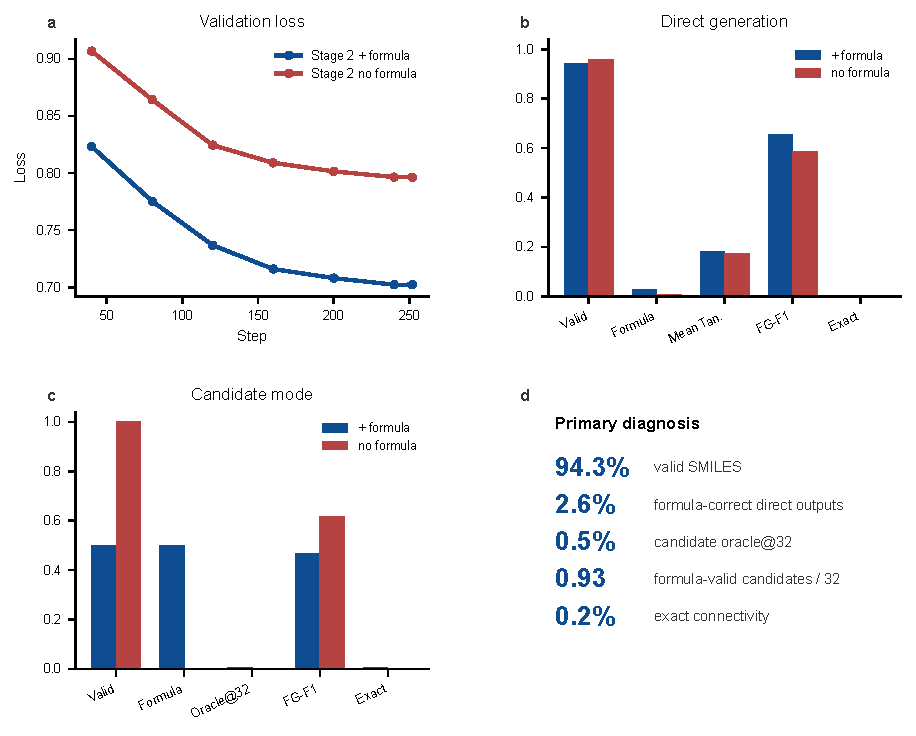
\includegraphics[width=\linewidth]{figures/fig2_results.pdf}
\caption{\textbf{Training and test-set outcomes.} \textbf{a}, Stage 2 validation loss curves for formula-conditioned and no-formula structure-only fine-tuning. \textbf{b}, Direct greedy generation metrics. \textbf{c}, Candidate-generation metrics after parsing, filtering, and reranking. \textbf{d}, Key diagnostic numbers for the formula-conditioned direct and candidate settings. Formula conditioning improves several soft metrics, but exact structure recovery remains limited by formula compliance and candidate recall.}
\label{fig:results}
\end{figure}

\subsection{Direct generation}

Table~\ref{tab:direct} reports direct greedy generation on the 1,000-sample test set. Both direct models emit valid molecules at high rates. The no-formula model slightly exceeds the formula model in valid-\smiles{} rate (95.7\% versus 94.3\%), but the formula model obtains better molecular formula accuracy, Tanimoto similarity, and functional-group F1. The formula-conditioned exact match is 0.2\%, corresponding to two exact connectivity matches out of 1,000 test examples. The no-formula exact match is zero.

\begin{table}[t]
\centering
\caption{Direct greedy inference on the 1,000-sample test split. Exact and connectivity exact are identical in these runs because targets are evaluated without stereochemistry.}
\label{tab:direct}
\scriptsize
\begin{tabular}{lcccccccc}
\toprule
Run & Exact & Valid & Formula acc. & Mean Tan. & Tan. \(\geq .3\) & FG micro-F1 & JSON ok & Unique \\
\midrule
Formula & 0.002 & 0.943 & 0.026 & 0.183 & 0.082 & 0.657 & 0.943 & 0.988 \\
No formula & 0.000 & 0.957 & 0.006 & 0.175 & 0.073 & 0.588 & 0.957 & 0.940 \\
\bottomrule
\end{tabular}
\end{table}

The soft metrics reveal partial learning. The formula-conditioned direct model reaches 65.7\% functional-group micro-F1 and 63.5\% sample-macro F1. In the per-class analysis, common and visually salient classes such as aromatic rings, organohalogens, silicon-carbon motifs, esters, ketones, and amides are learned better than rare classes such as aldehydes, nitro groups, sulfoxides, and carboxylic acids. This pattern is consistent with the model learning local chemical regularities and frequency-dependent priors rather than complete global structure.

The failure mode is formula inconsistency. Only 2.6\% of valid formula-conditioned direct outputs match the reference formula, even though the formula is explicitly present in the prompt. The model therefore treats the formula as a useful textual hint but not as a hard constraint. This finding is important because it explains why exact match remains low despite valid outputs. If the atom counts or heteroatom composition are wrong, the prediction cannot be an exact structural match regardless of local spectral plausibility.

\subsection{Candidate generation and reranking}

Candidate inference was intended to improve over greedy decoding by sampling 32 possible structures, filtering them, pre-sorting them with rule evidence, and asking the model to select the best candidate. Table~\ref{tab:candidates} shows that this version does not yet solve the problem. Formula-conditioned candidate inference reaches 50.0\% molecular formula accuracy because formula-mismatched predictions are filtered out, but half of the test examples have zero formula-valid candidates and therefore produce an empty final prediction. Mean formula-valid candidate count is only 0.93 out of 32 sampled completions.

\begin{table}[t]
\centering
\caption{Top-32 candidate inference. Oracle@32 measures whether the reference structure appears in the selectable candidate set after parsing, canonicalization, and filtering.}
\label{tab:candidates}
\scriptsize
\setlength{\tabcolsep}{3pt}
\begin{tabular}{@{}lcccccccc@{}}
\toprule
Run & Exact & Valid & Formula & Oracle & Mean FV & Filter fail & Rank try & Rank fail \\
\midrule
Formula & 0.004 & 0.500 & 0.500 & 0.005 & 0.93 & 0.500 & 0.233 & 0.021 \\
No formula & 0.000 & 1.000 & 0.003 & 0.001 & 0.00 & 0.000 & 1.000 & 0.159 \\
\bottomrule
\end{tabular}
\end{table}

The decisive number is oracle@32. In the formula-conditioned setting, the reference connectivity appears in the filtered top-32 candidate set for only 0.5\% of test examples. In the no-formula setting, the corresponding rate is 0.1\%. A reranker cannot recover the correct structure if it is absent from the candidate set. The current candidate results therefore diagnose candidate generation rather than candidate ranking. The LLM samples many valid molecules, but the formula-valid and reference-covering subset is too small.

This result also clarifies the role of the NMR rule library. Rule-based pre-sorting can help choose among chemically plausible candidates, but it cannot create a missing candidate. Future improvements should first raise formula-valid candidate recall through constrained decoding, formula-aware molecular generation, retrieval from a molecular index, or graph-based proposal mechanisms. Only after oracle@\(k\) becomes nontrivial can reranking quality be meaningfully evaluated.

\begin{figure}[t]
\centering
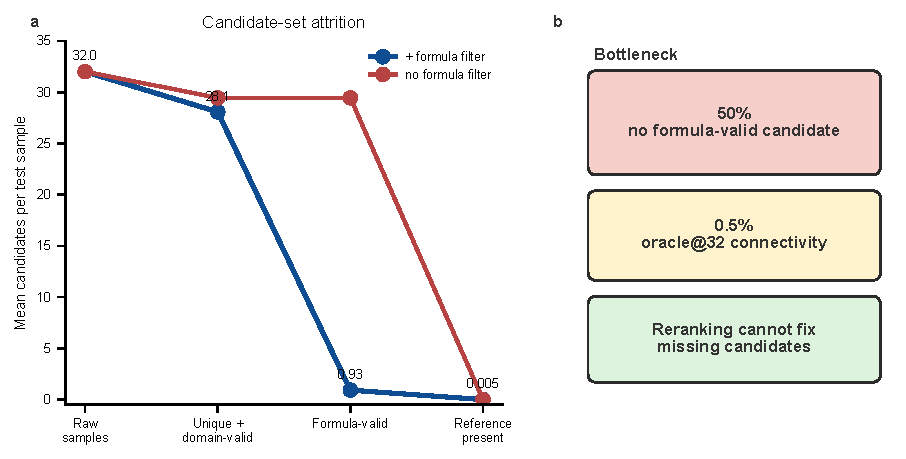
\includegraphics[width=\linewidth]{figures/fig3_candidate_bottleneck.pdf}
\caption{\textbf{Candidate-generation bottleneck.} \textbf{a}, Mean candidate counts through parsing, domain filtering, formula filtering, and reference-presence checks. Formula filtering removes most sampled structures; the correct reference appears in the selectable formula-conditioned set for only 0.5\% of test examples. \textbf{b}, Practical implication: the present bottleneck is recall of formula-valid candidates, not the reranker.}
\label{fig:candidate-bottleneck}
\end{figure}

\subsection{Interpretation of model behavior}

The direct and candidate results together support three conclusions. First, text LLM fine-tuning is effective at output formatting and local chemical pattern learning. The model learns the JSON schema, produces valid molecules, and predicts many broad functional groups better than chance. Second, exact NMR-to-structure prediction is much harder than producing a plausible molecule. Small changes in ring size, heteroatom placement, or substituent connectivity can leave broad 1D NMR features similar while changing the exact \smiles{} target. Third, formula information must be enforced algorithmically. A model that receives the formula as text can still output a chemically valid molecule with the wrong formula.

These observations are consistent with the known ambiguity of one-dimensional NMR. Without 2D correlations, mass spectrometry, infrared evidence, or a database of candidate structures, many molecules can share overlapping chemical-shift patterns. The appropriate claim for the current system is therefore not autonomous structure elucidation. It is a benchmark and diagnostic framework showing where a text LLM helps and where deterministic chemical constraints remain necessary.

\subsection{Why the final study is text-only}

The project originally considered rendered spectrum images and a vision-language model. The final study intentionally removes that component. This decision is supported by both practical and scientific considerations. Practically, rendering and loading paired spectrum images dominated throughput, while the model still needed peak tables for stable interpretation. Scientifically, the available synthetic data are already structured as peak measurements. If the central question is whether a foundation model can use routine 1D NMR evidence, then a text LLM over peak tables is the cleanest first test. It avoids confounding the experiment with image resolution, plot styling, axis rendering, antialiasing, and visual-token budget.

This does not mean that spectral images are useless. Images may matter when peak picking is uncertain, when line shapes, baselines, impurities, or integration traces contain information absent from a table, or when the goal is end-to-end interpretation from instrument output. Those conditions are outside the present data regime. The current dataset contains simulated peak tables without solvent peaks, and the strongest failure is not visual perception. The failure is that unconstrained generation rarely produces the correct formula-valid molecular graph. A VLM would not automatically solve that bottleneck unless it also improved chemically constrained candidate recall.

\section{Discussion}

\subsection{What the model has learned}

The strongest positive evidence is the gap between exact correctness and functional-group performance. A model that merely memorized token statistics would not reliably distinguish broad structural classes. The formula-conditioned direct model detects aromatic rings, organohalogens, silicon-carbon motifs, esters, ketones, and amides at useful rates. These groups are plausible because they produce recurring signatures in chemical shifts and atom environments. For example, aromatic systems shift both \(^{1}\)H and \(^{13}\)C signals downfield, carbonyl-containing groups affect \(^{13}\)C regions, and organohalogens or silicon groups constrain composition when a formula is present.

This local learning is still insufficient for exact connectivity. 1D NMR peak tables compress the full spectrum into a small set of signals. Equivalent environments, overlapping multiplets, missing exchangeable protons, and ambiguous substitution patterns all reduce information. Even when the model predicts the correct functional groups, it may place them on the wrong scaffold or choose the wrong isomer. The low ring-scaffold match rate indicates that the model's global graph construction is weak.

\subsection{Why formula conditioning helps but does not solve the task}

Formula conditioning lowers validation loss and improves direct Tanimoto and functional-group F1, but formula accuracy remains poor under direct decoding. This is a standard failure mode for language models asked to obey symbolic constraints. The formula appears in the prompt as text, while generation proceeds token by token without a decoder-level check that atom counts remain feasible. The model can produce a chemically valid continuation that is statistically likely under the learned distribution but inconsistent with the exact formula.

Hard filtering fixes part of this issue. In candidate mode, the formula-conditioned final predictions all either match the formula or are empty after filtering, which raises formula accuracy among non-empty outputs. However, filtering also exposes the lack of formula-valid proposals. Half of the test examples have no formula-valid sampled candidate among 32 completions. Thus, formula constraints are necessary but not sufficient. The candidate generator itself must become formula aware.

\subsection{Implications for future systems}

The results suggest a staged architecture for future work. A text LLM can provide instruction following, prompt flexibility, and local NMR reasoning. Deterministic chemistry code should enforce molecule validity, allowed elements, charge neutrality, isotope policy, and formula consistency. A separate candidate proposal mechanism should ensure high recall under these constraints. Finally, NMR rules or a learned reranker can select among plausible candidates. This architecture is closer to how human spectroscopists work: they do not freely write arbitrary structures; they constrain possible structures by formula, unsaturation, atom environments, and compatibility with observed signals.

The next experimental gate should therefore be candidate oracle@\(k\), not top-1 exact match. If oracle@32 remains below 1\%, reranking experiments are not informative. A useful intermediate target is to raise formula-valid candidate count and candidate oracle@\(k\) while keeping output diversity high. Candidate proposals could come from formula-indexed molecular retrieval, fragment assembly, grammar-constrained \smiles{} decoding, graph-generation models, or hybrid LLM-plus-enumerator procedures. Once the correct structure appears in the candidate set at meaningful frequency, rule-based and model-based ranking can be evaluated separately.

A practical next system would combine four components. First, formula-indexed retrieval would provide a pool of known molecules with exact atom counts, making the candidate set immediately formula-valid when the target lies within the database. Second, formula-constrained generation would propose molecules outside that database while rejecting impossible partial strings during decoding. Third, rule and spectrum-simulation scores would remove candidates whose functional groups contradict the observed \(^{1}\)H/\(^{13}\)C regions. Fourth, an LLM or smaller cross-encoder would rank the surviving set using the full peak table. This architecture changes the LLM's role from unconstrained molecule inventor to evidence-aware selector, a role more consistent with the observed strengths of the present model.

The results also suggest how to scale the data. Simply expanding from 10k to hundreds of thousands of examples may lower loss and improve functional-group coverage, but it should be paired with constraint-aware inference metrics. A larger dataset should be judged by whether it raises formula accuracy, formula-valid candidate count, and oracle@\(k\), not only by whether it improves valid-\smiles{} rate. Otherwise, training may produce a better chemical language model without producing a better structure elucidation system.

\section{Limitations}

This study has several limitations. The first is dataset scale. Although the raw project data are large, the reported pilot uses only 10k curated examples. More data may improve local spectral associations and output format stability, but it is unlikely to remove the need for hard constraints because formula consistency is a decoding property, not only a data-size property.

The second limitation is the absence of external modalities. The experiments use only 1D \(^{1}\)H/\(^{13}\)C peak tables and optional formula. They do not use 2D NMR, infrared spectra, mass spectra, solvent peaks, impurities, raw free induction decays, or rendered spectrum images. The conclusions therefore apply to structured 1D peak-table inputs, not to full manual structure elucidation.

The third limitation is target identifiability. Exact \smiles{} matching treats the dataset reference as unique, but one-dimensional NMR may not uniquely distinguish constitutional isomers in all cases. A low exact-match rate is partly a model failure, but the task definition itself is strict. Reporting Tanimoto, scaffold, functional-group F1, formula accuracy, and candidate oracle metrics helps expose partial progress without pretending that every 1D spectrum has a unique answer.

The fourth limitation is that the current rule library has not yet been tested as prompt context. The reported runs set \texttt{rule\_context\_enabled=false}. Therefore, the paper does not claim that textual rule evidence improves training. The rule library is used for analysis and post-generation candidate pre-sorting, and its training-time value remains an ablation to run later.

\section{Conclusion}

\spectralm{} provides a text-only LLM framework for studying molecular structure prediction from paired \(^{1}\)H and \(^{13}\)C NMR peak tables. The framework includes data curation, JSON-constrained instruction tuning, response-only supervision, formula/no-formula ablations, candidate generation, formula/domain filtering, NMR-rule pre-ranking, and multi-level evaluation. The central result is diagnostic: Qwen3-8B adapters can learn to emit valid molecules and capture partial functional-group information from 1D NMR peak tables, but direct exact connectivity prediction remains near zero in the current 10k pilot. Formula helps, but only as a soft prompt cue unless enforced by post-generation chemistry. Candidate reranking is not yet useful because candidate oracle recall is too low.

These findings redirect the research program. The next step is not simply larger training or a more elaborate reranker. The system needs a candidate generator that reliably proposes diverse, formula-valid structures. Once oracle recall improves, NMR rules and learned ranking can be evaluated as genuine structure-selection mechanisms. In this sense, \spectralm{} is best viewed as a transparent benchmark and failure-analysis platform for text LLMs in NMR structure elucidation.

\section*{Ethics, Data Availability, and AI Disclosure}

This work uses molecular structure and spectral data and does not involve human subjects, clinical records, or personal data. The curated benchmark construction scripts, training code, evaluation code, and experiment configurations are contained in the project repository. Redistribution of the raw CSV source should follow the license and provenance constraints of the original dataset. The reported predictions and summaries are stored under \texttt{outputs/experiments/structure/predictions/}. This manuscript draft was prepared with assistance from an AI coding and writing tool under author direction. The author is responsible for verifying all claims, references, numerical results, and final wording before submission.

\begin{ack}
The author thanks the maintainers of RDKit, PyTorch, Hugging Face Transformers, TRL, PEFT, and Unsloth for open-source infrastructure used in the project. The current results should be interpreted as a pilot study and failure analysis rather than a production-ready structure elucidation system.
\end{ack}

\section*{References}

{\small
\begin{thebibliography}{99}

\bibitem{Alberts2023}
Marvin Alberts, Federico Zipoli, and Alain C. Vaucher.
Learning the language of NMR: Structure elucidation from NMR spectra using transformer models.
ChemRxiv preprint, 2023.

\bibitem{Alberts2025}
Marvin Alberts, Nina Hartrampf, and Teodoro Laino.
Automated structure elucidation at human-level accuracy via a multimodal multitask language model.
ChemRxiv preprint, 2025.

\bibitem{Bemis1996}
Guy W. Bemis and Mark A. Murcko.
The properties of known drugs. 1. Molecular frameworks.
\textit{Journal of Medicinal Chemistry}, 39(15):2887--2893, 1996.

\bibitem{Breitmaier2002}
Eberhard Breitmaier.
\textit{Structure Elucidation by NMR in Organic Chemistry: A Practical Guide}.
Wiley, 3rd edition, 2002.

\bibitem{Claridge2016}
Timothy D. W. Claridge.
\textit{High-Resolution NMR Techniques in Organic Chemistry}.
Elsevier, 3rd edition, 2016.

\bibitem{Dettmers2023QLoRA}
Tim Dettmers, Artidoro Pagnoni, Ari Holtzman, and Luke Zettlemoyer.
QLoRA: Efficient finetuning of quantized LLMs.
In \textit{Advances in Neural Information Processing Systems}, 2023.

\bibitem{Devata2024}
Sriram Devata, Bhuvanesh Sridharan, Sarvesh Mehta, Yashaswi Pathak, Siddhartha Laghuvarapu, Girish Varma, and U. Deva Priyakumar.
DeepSPInN: Deep reinforcement learning for molecular structure prediction from infrared and \(^{13}\)C NMR spectra.
2024.

\bibitem{Ernst1987}
Richard R. Ernst, Geoffrey Bodenhausen, and Alexander Wokaun.
\textit{Principles of Nuclear Magnetic Resonance in One and Two Dimensions}.
Oxford University Press, 1987.

\bibitem{Hu2021LoRA}
Edward J. Hu, Yelong Shen, Phillip Wallis, Zeyuan Allen-Zhu, Yuanzhi Li, Shean Wang, Lu Wang, and Weizhu Chen.
LoRA: Low-rank adaptation of large language models.
arXiv:2106.09685, 2021.

\bibitem{Hu2024}
Frank Hu, Michael S. Chen, Grant M. Rotskoff, Matthew W. Kanan, and Thomas E. Markland.
Accurate and efficient structure elucidation from routine one-dimensional NMR spectra using multitask machine learning.
\textit{ACS Central Science}, 10:2162--2170, 2024.

\bibitem{Huang2021}
Zhaorui Huang, Michael S. Chen, Cristian P. Woroch, Thomas E. Markland, and Matthew W. Kanan.
A framework for automated structure elucidation from routine NMR spectra.
2021.

\bibitem{Jin2026}
Yongqi Jin, Jun-Jie Wang, Fanjie Xu, Xiaohong Ji, Zhifeng Gao, Linfeng Zhang, Guolin Ke, Rong Zhu, and Weinan E.
NMR-Solver: Automated structure elucidation via large-scale spectral matching and physics-guided fragment optimization.
\textit{Nature Communications}, 2026.

\bibitem{Kingma2015}
Diederik P. Kingma and Jimmy Ba.
Adam: A method for stochastic optimization.
In \textit{International Conference on Learning Representations}, 2015.

\bibitem{Levitt2008}
Malcolm H. Levitt.
\textit{Spin Dynamics: Basics of Nuclear Magnetic Resonance}.
Wiley, 2nd edition, 2008.

\bibitem{Liu2025}
Shiyun Liu and Jacqueline M. Cole.
Automated determination of the molecular substructure from nuclear magnetic resonance spectra using neural networks.
\textit{Journal of Chemical Information and Modeling}, 65:8435--8447, 2025.

\bibitem{Loshchilov2019}
Ilya Loshchilov and Frank Hutter.
Decoupled weight decay regularization.
In \textit{International Conference on Learning Representations}, 2019.

\bibitem{Mangrulkar2022}
Sourab Mangrulkar, Sylvain Gugger, Lysandre Debut, Younes Belkada, Sayak Paul, and Benjamin Bossan.
PEFT: State-of-the-art parameter-efficient fine-tuning methods.
\url{https://github.com/huggingface/peft}, 2022.

\bibitem{Morgan1965}
Harry L. Morgan.
The generation of a unique machine description for chemical structures: A technique developed at Chemical Abstracts Service.
\textit{Journal of Chemical Documentation}, 5(2):107--113, 1965.

\bibitem{Paszke2019}
Adam Paszke, Sam Gross, Francisco Massa, Adam Lerer, James Bradbury, Gregory Chanan, Trevor Killeen, Zeming Lin, Natalia Gimelshein, Luca Antiga, and others.
PyTorch: An imperative style, high-performance deep learning library.
In \textit{Advances in Neural Information Processing Systems}, 2019.

\bibitem{Pretsch2009}
Ern{\"o} Pretsch, Philippe B{\"u}hlmann, and Martin Badertscher.
\textit{Structure Determination of Organic Compounds: Tables of Spectral Data}.
Springer, 4th edition, 2009.

\bibitem{QwenTeam2025}
Qwen Team.
Qwen3 technical report.
arXiv preprint, 2025.

\bibitem{RDKit}
Greg Landrum.
RDKit: Open-source cheminformatics software.
\url{https://www.rdkit.org/}, 2016.

\bibitem{Rogers2010}
David Rogers and Mathew Hahn.
Extended-connectivity fingerprints.
\textit{Journal of Chemical Information and Modeling}, 50(5):742--754, 2010.

\bibitem{Silverstein2014}
Robert M. Silverstein, Francis X. Webster, David J. Kiemle, and David L. Bryce.
\textit{Spectrometric Identification of Organic Compounds}.
Wiley, 8th edition, 2014.

\bibitem{Sridharan2022}
Bhuvanesh Sridharan, Sarvesh Mehta, Yashaswi Pathak, and U. Deva Priyakumar.
Deep reinforcement learning for molecular inverse problem of nuclear magnetic resonance spectra to molecular structure.
\textit{Journal of Physical Chemistry Letters}, 13:4924--4933, 2022.

\bibitem{Tanimoto1958}
Taffee T. Tanimoto.
An elementary mathematical theory of classification and prediction.
IBM Internal Report, 1958.

\bibitem{Vaswani2017}
Ashish Vaswani, Noam Shazeer, Niki Parmar, Jakob Uszkoreit, Llion Jones, Aidan N. Gomez, Lukasz Kaiser, and Illia Polosukhin.
Attention is all you need.
In \textit{Advances in Neural Information Processing Systems}, 2017.

\bibitem{VonWerra2020}
Leandro von Werra, Younes Belkada, Lewis Tunstall, Edward Beeching, Tristan Thrush, Nathan Lambert, Shengyi Huang, Kashif Rasul, and Quentin Gallou{\'e}dec.
TRL: Transformer reinforcement learning.
\url{https://github.com/huggingface/trl}, 2020.

\bibitem{Weininger1988}
David Weininger.
SMILES, a chemical language and information system. 1. Introduction to methodology and encoding rules.
\textit{Journal of Chemical Information and Computer Sciences}, 28(1):31--36, 1988.

\bibitem{Wolf2020}
Thomas Wolf, Lysandre Debut, Victor Sanh, Julien Chaumond, Clement Delangue, Anthony Moi, Pierric Cistac, Tim Rault, R{\'e}mi Louf, Morgan Funtowicz, Joe Davison, Sam Shleifer, Patrick von Platen, Clara Ma, and others.
Transformers: State-of-the-art natural language processing.
In \textit{Proceedings of the 2020 Conference on Empirical Methods in Natural Language Processing: System Demonstrations}, pages 38--45, 2020.

\bibitem{Xiong2025}
Ziyu Xiong, Yichi Zhang, Foyez Alauddin, Chu Xin Cheng, Joon Soo An, Mohammad R. Seyedsayamdost, and Ellen D. Zhong.
Atomic diffusion models for small molecule structure elucidation from NMR spectra.
Preprint, 2025.

\bibitem{Yang2025}
Qingsong Yang, Binglan Wu, Xuwei Liu, Bo Chen, Wei Li, Gen Long, Xin Chen, and Mingjun Xiao.
DiffNMR: Diffusion models for nuclear magnetic resonance spectra elucidation.
Preprint, 2025.

\bibitem{Yang2026}
Liujia Yang, Zhuo Yang, Jiaqing Xie, Yubin Wang, Ben Gao, Xingjian Wei, Jiaxing Sun, Tianfan Fu, Jiang Wu, Conghui He, and Yuqiang Li.
NMRTrans: Structure elucidation from experimental NMR spectra via set transformers.
Preprint, 2026.

\bibitem{Yao2023}
Lin Yao, Minjian Yang, Jianfei Song, Zhuo Yang, Hanyu Sun, Hui Shi, Xue Liu, Xiangyang Ji, Yafeng Deng, and Xiaojian Wang.
Conditional molecular generation net enables automated structure elucidation based on \(^{13}\)C NMR spectra and prior knowledge.
\textit{Analytical Chemistry}, 95:5393--5401, 2023.

\end{thebibliography}
}

\end{document}
